\documentclass[compress]{beamer}
%\usetheme{Montpellier}
%\usecolortheme{dove}
%\useinnertheme{rounded}
%\useoutertheme{smoothbars}
\usetheme{Madrid}
\usefonttheme{serif}
\usecolortheme{dove}
\useinnertheme{rounded}
\useoutertheme{miniframes}
\setbeamersize{text margin left=5mm,text margin right=10mm}
\usepackage{graphicx}
\usepackage{multicol}
\setbeamertemplate{navigation symbols}[horizontal] 
\setbeamersize{text margin left=5mm,text margin right=5mm} 
\setbeamercolor{subsection name}{fg=white}
\setbeamercolor{section name}{fg=white}
\usepackage{xcolor}
\usepackage{tikz}
\usepackage[absolute,overlay]{textpos}
\usepackage{spot}
\usepackage{tikzsymbols}
\usetikzlibrary{mindmap,calc,patterns,decorations.pathmorphing,decorations.markings, arrows, shapes.arrows, shapes, backgrounds}
\definecolor{unipd}{RGB}{155, 0, 20}
\definecolor{grigioPantano}{RGB}{72,79,89}


\setbeamerfont{block title}{family=\bfseries}
\setbeamercolor{block title}{use=structure,fg=unipd,bg=white}
%\setbeamercolor{block body}{fg=black,use=block title,bg=grigioPantano!10}
%
%
%\setbeamercolor{block title example}{use=example text,fg=white,bg=green!50!black}
%\setbeamercolor{block body example}{fg=grigioPantano!60!black,use=block title example,bg=grigioPantano!10}
%
%\setbeamercolor{block title alerted}{use=alerted text,fg=white,bg=unipd}
%\setbeamercolor{block body alerted}{fg=black,use=block title alerted,bg=grigioPantano!20}


  \tikzset{
	invisible/.style={opacity=0},
	visible on/.style={alt={#1{}{invisible}}},
	alt/.code args={<#1>#2#3}{%
		\alt<#1>{\pgfkeysalso{#2}}{\pgfkeysalso{#3}} % \pgfkeysalso doesn't change the path
	},
	every overlay node/.style={
		%draw=black,fill=white,rounded corners,
		anchor=north west, inner sep=0pt,
	},
}

 \title[Randomness and possibilities]{When randomness opens new possibilities: Acknowledging the stimulus sampling variability in Experimental Psychology}
\vspace{-1.5mm}\author[OME, PA, ER]{ Ottavia M. Epifania\textsuperscript{1,2,3}, Pasquale Anselmi\textsuperscript{1}, Egidio Robusto\textsuperscript{1}\\ \texttt{ottavia.epifania@unipd.it}}
\institute[]{\small \textsuperscript{1} University of Padova (IT) \\
\textsuperscript{2} Psicostat Group \\
\textsuperscript{3} Catholic Univerisity of the Sacred Heart, Milan (IT) \\}
\vspace*{-5mm}
\date[CMS Conference]{\footnotesize Conference CMS Berlin \\ December 16}
\titlegraphic{\vspace{-5mm}%
	
\includegraphics[width=1.5cm,height=1.5cm,keepaspectratio]{img/unipd.png}%\hspace*{9.75cm}~%
	
\includegraphics[width=2cm,height=2cm,keepaspectratio]{img/psicostat.png}%
	
\includegraphics[width=1.5cm,height=1.5cm,keepaspectratio]{img/unicatt.png}%
}

\definecolor{back}{RGB}{247, 251, 255}
\definecolor{map}{RGB}{111, 172, 232}
\definecolor{childmap}{RGB}{161, 200, 240}
\definecolor{nodemap}{RGB}{141, 170, 199}
\definecolor{rasch}{rgb}{0.0, 0.33, 0.71}
\definecolor{log}{rgb}{0.0, 0.65, 0.58}
\definecolor{diff}{RGB}{33, 113, 181}
\definecolor{single}{RGB}{106, 81, 163}
\definecolor{comp}{RGB}{35, 99, 70}
\definecolor{inc}{RGB}{191, 13, 43}
\definecolor{highlight}{rgb}{0.45, 0.31, 0.59}
\definecolor{section}{RGB}{51,51,179}
\definecolor{typical}{RGB}{8, 69, 148}
\definecolor{model}{RGB}{74, 20, 134}
\definecolor{orangered2}{RGB}{238,64,0}
\definecolor{royalblue3}{RGB}{58,95,205}
\definecolor{springgreen}{RGB}{0,205,102}
\definecolor{magenta}{RGB}{255,0,255}
\def\tikzoverlay{%
	\tikz[remember picture, overlay]\node[every overlay node]
}%

%\AtBeginSubsection{\frame{\subsectionpage}}
 
\setbeamertemplate{subsection page}
{
	\begingroup
	\begin{beamercolorbox}[sep=12pt,center]{section title}
		\usebeamerfont{section title}\insertsection\par
	\end{beamercolorbox}
	\vspace*{5pt}
	\begin{beamercolorbox}[sep=8pt,center]{subsection title}
		\usebeamerfont{subsection title}\insertsubsection\par
	\end{beamercolorbox}
	\endgroup
}

\begin{document}
\begin{frame}[plain]
%    \maketitle
\begin{center}
		\large \bfseries When randomness opens new possibilities: \\ Acknowledging the stimulus sampling variability in Experimental Psychology
\end{center}

\vspace{2.5mm}
\begin{center}
	\textbf{Ottavia M. Epifania}\textsuperscript{1,2,3}, Pasquale Anselmi\textsuperscript{1}, Egidio Robusto\textsuperscript{1}
	
	\vspace{1.5mm}
	
	\begin{columns}[T]
		\begin{column}{.33\linewidth}
			\centering 	
\includegraphics[width=1.5cm,height=1.5cm,keepaspectratio]{img/unipd.png}
		\end{column}
		\begin{column}{.33\linewidth}
			\centering 
\includegraphics[width=2.5cm,height=2.5cm,keepaspectratio]{img/psicostat.png}
		\end{column}
		\begin{column}{.33\linewidth}
			\centering  
\includegraphics[width=1.5cm,height=1.5cm,keepaspectratio]{img/unicatt.png}
		\end{column}
	\end{columns}
	
	\end{center}
	
	\vspace{1.5mm}
	
	\begin{center}
	\small \textsuperscript{1} University of Padova (IT) \\
	\textsuperscript{2} Psicostat Group, University of Padova (IT) \\
	\textsuperscript{3} Università Cattolica del Sacro Cuore, Milan (IT) \\
\end{center}

\vspace{5mm}



\end{frame}



\section{Introduction}

\subsection{Stimuli are fixed, respondents are random}

\begin{frame}
	
	\begin{block}{Respondents are random}
		
		Sampled from a larger population
		
		\vspace{1.5mm}
		\pause
		Need for acknowledging the sampling variability 
		
		\vspace{1.5mm}
		\pause
		Results can be generalized to other respondents belonging to the same population
	\end{block}

\vspace{3mm}
\pause
\begin{block}{Stimuli/item are fixed}
	
	Taken to be entire population 
	
		\vspace{1.5mm}
	\pause
	There is no sampling variability
	
		\vspace{1.5mm}
	\pause
	There is no need to generalize the results because the stimuli are the population
	
\end{block}
\end{frame}

\begin{frame}{However...}
	
	The stimuli can also represent a sample of a larger universe
	
	\vspace{3mm}
	\pause
	
	\begin{exampleblock}{Processing speed of positive and negative attributes}
		
		\pause
		\vspace{1.5mm}
		There is a universe of {\color{rasch}{\textbf{positive attributes}}} as well as an universe of {\color{unipd}{\textbf{negative attributes}}}
		
		\pause
		\vspace{1.5mm}
		Only samples of {\color{rasch}{\textbf{positive attributes}}} (e.g., good, nice, $\ldots$) and {\color{unipd}{\textbf{negative attributes}}} (e.g., bad, evil, $\ldots$) are administered 
		
		\pause
		\vspace{2.5mm}
		So... \textbf{there must be a sampling variability!} 
	\end{exampleblock}
\end{frame}

\subsection{What if the sampling variability is not acknowledged}

\begin{frame}{}
	
	
	\begin{block}{Generalizability}
	
	\small
	
	Generalizability is bounded to the specific set of stimuli used in the experiment
	 
	 Results can be generalized if and only if the exact same set of stimuli is used 
	

	\end{block}
	
	\pause
 
	\begin{block}{Robustness of the results}
		
		\small
		Random variability at the stimulus level might inflate the probability of committing Type I errors
		
		Averaging across stimuli to obtain person-level scores results in biased estimates due to the noise in the data
	\end{block}
	
	\pause
	
	\begin{block}{Loss of information}
		
		\small
		Every stimulus is assumed to be equally informative
		
		All the variability is not considered as well as all the information that can be obtained from it 
	\end{block}
	
\end{frame}

\begin{frame}{This contribution}
	Focus on the loss of information...the other side of the coin 
	
	\vspace{2.5mm}
	\pause
	The information at the stimulus level that can be retrieved from the accuracy responses (correct vs. incorrect) from a typical experiment where the response times are usually employed for scoring the data
	
	\vspace{2.5mm}
	\pause 
	It can actually help in disentangling what is known to be a shortcoming of the score usually employed for analyzing the data of this experiment
\end{frame}

\section{Random effects for random factors}

\begin{frame}{Generalized linear model for dichotomous responses}
	
	\begin{figure}
		\begin{overprint}
			\onslide<1>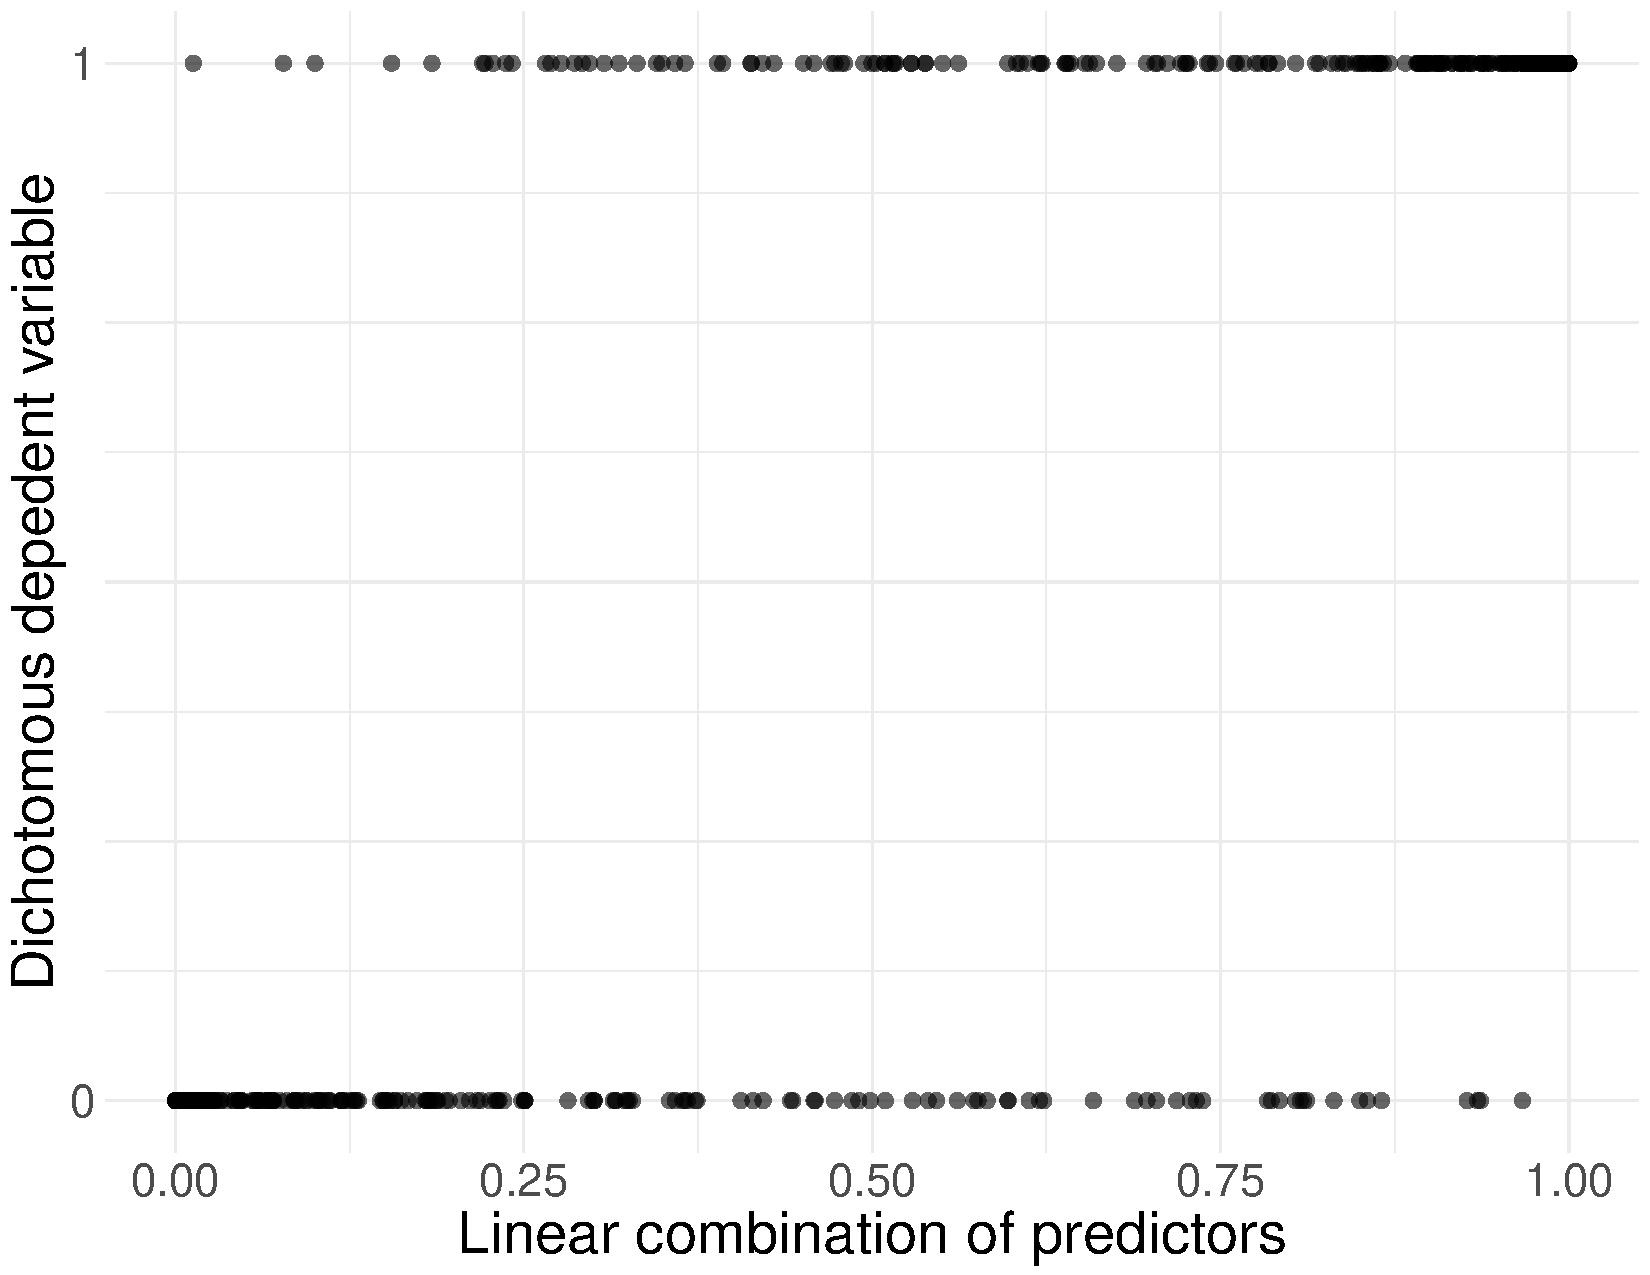
\includegraphics[width=0.7\linewidth]{img/baseGLM.pdf}
			\onslide<2>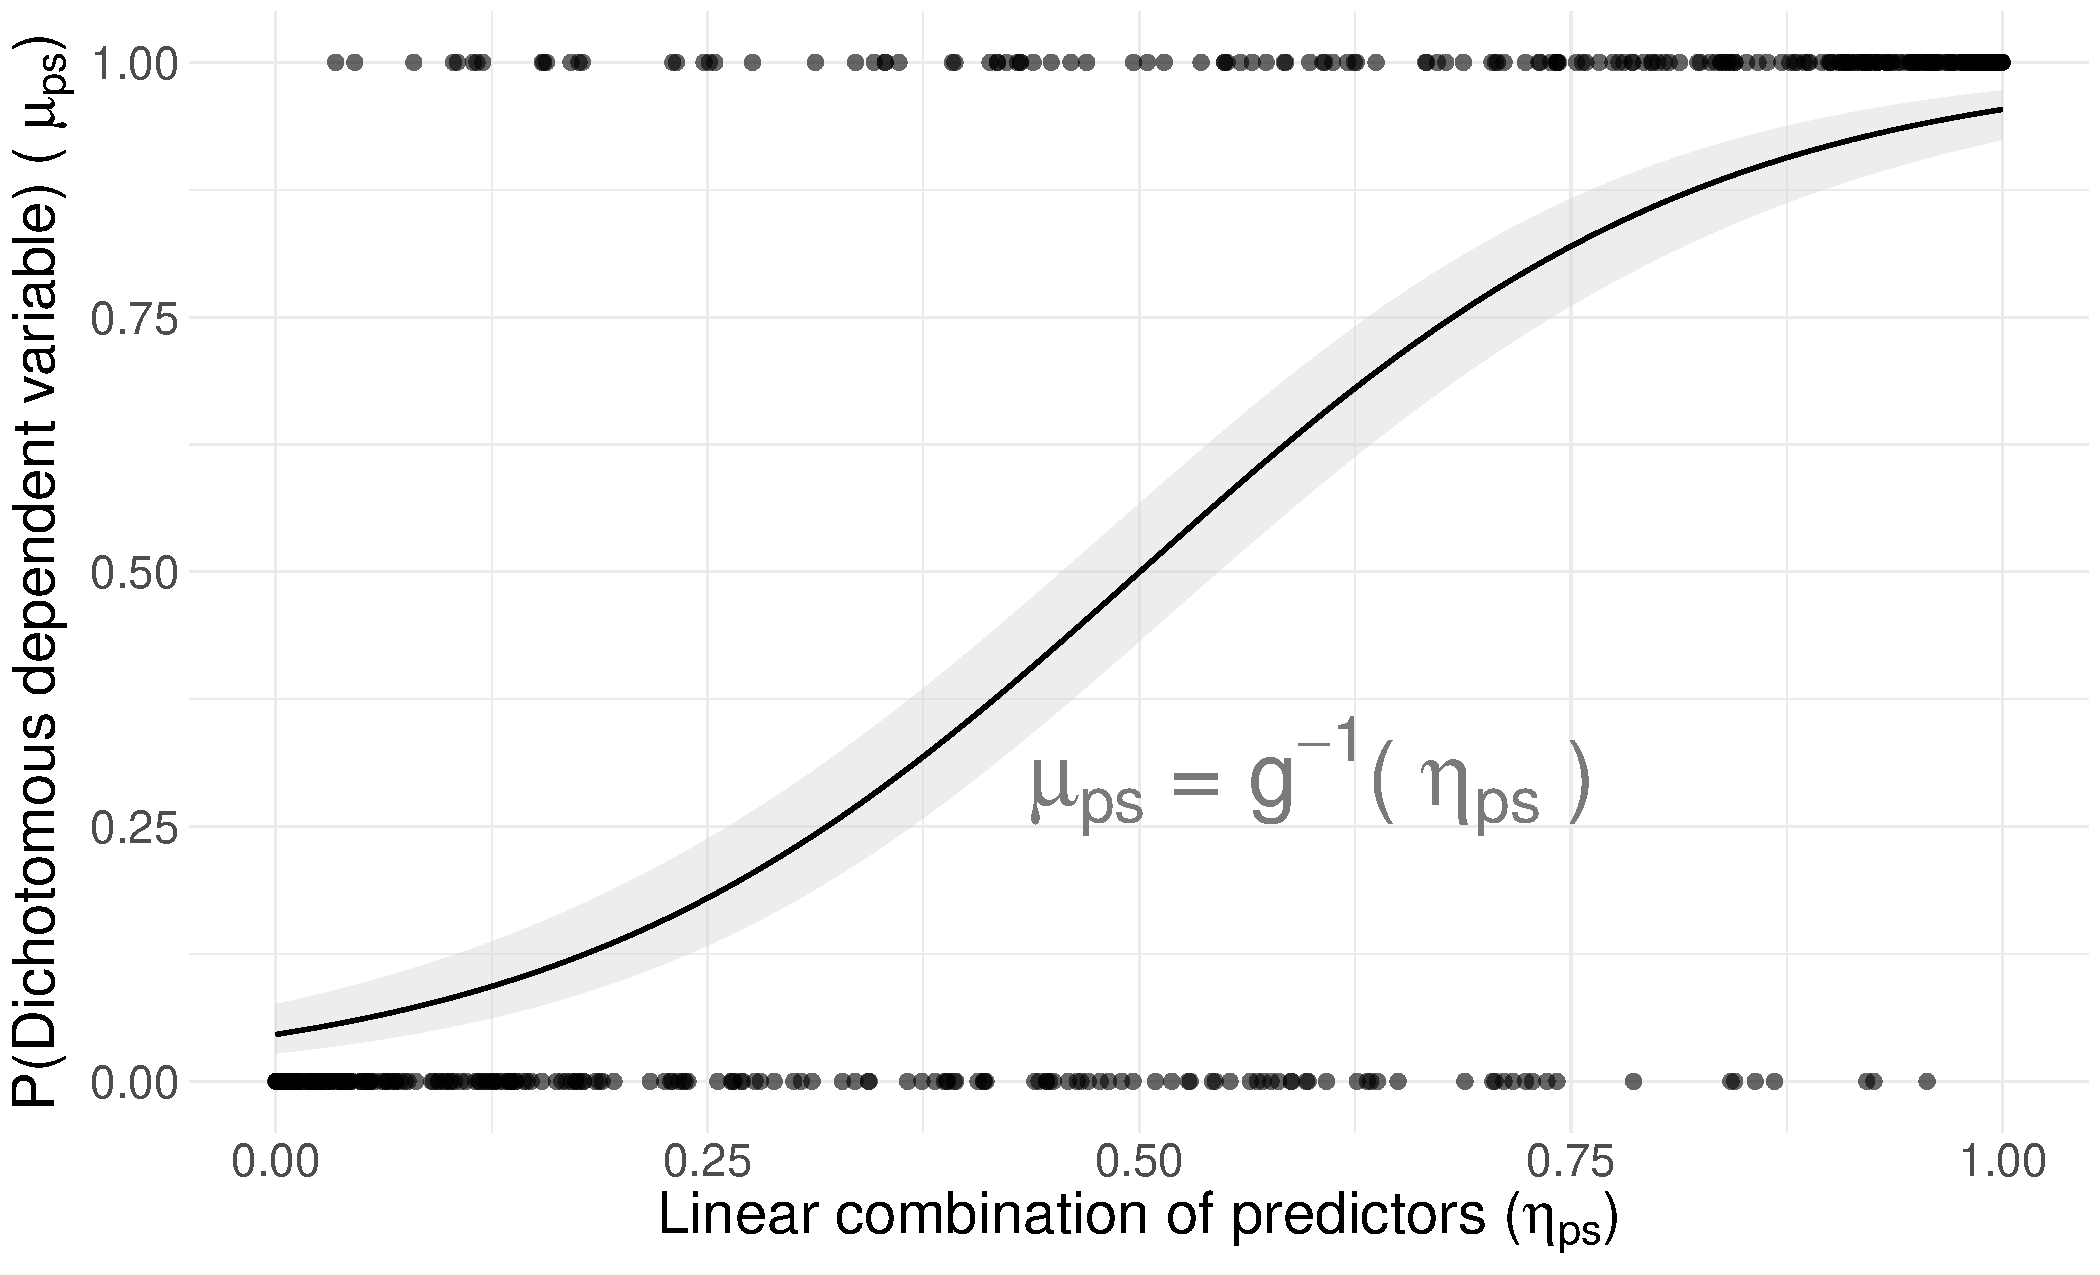
\includegraphics[width=0.7\linewidth]{img/linkGLM.pdf}
		\end{overprint}
	\end{figure}
	
	\onslide<2->
	\tikzoverlay (n1) at (8cm, 5.6cm){%
		\begin{minipage}{0.7\linewidth}
			
			\emph{Logit link function g}
			
			$g(\eta_{ps}) = log\left(\frac{\mu_{ps}}{1 - \mu_{ps}}\right)$
			
			\vspace{5mm}
			
			\emph{Inverse} $g^{-1}$
			
			\vspace{5mm}
			
			$g^{-1} = \frac{\exp(\eta_{ps})}{1 + \exp(\eta_{ps})} $
			
			\vspace{1.5mm}
		%	where $\eta_{ps} = \theta_p + b_s$
		\end{minipage}
	}; 
	
\end{frame}

\begin{frame}{Random effects and random factors}
	Linear component in a (G)LM: 
	\begin{equation}
		\eta = \beta X,
	\end{equation}
	where $\beta$ indicates the coefficients of the fixed intercept and slope(s), and $X$ is the model-matrix.
	
	Linear components in a (Generalized) Linear Mixed-Effects Model (GLMM): 
	
	\begin{equation}
		\eta = \beta X \, Zd,
	\end{equation}
	where $Z$ is the matrix and $d$ is the vector of the random effects (not parameters!)
	
	\onslide<2->
	
	\vspace{2.5mm}
	\begin{center}
		\emph{Best Linear Unbiased Predictors}
	\end{center}
\end{frame}

\begin{frame}{The Rasch model}
	\begin{equation*}
		P(x_{ps} = 1| \theta_p, b_s) = \dfrac{\exp( \theta_p - b_s)}{1 + \exp(\theta_p - b_s)}
	\end{equation*}
	where: 
	
	$\theta_p$: ability of respondent $p$ (i.e., latent trait level of respondent $p$)\\
	$b_s$: difficulty of stimulus $s$ (i.e., "challenging" power of stimulus $s$)\\
	
	\vspace{2.5mm}
	\onslide<2-> 
	\begin{columns}[T] % align columns
		\begin{column}{.50\linewidth}
			\textcolor{diff}{\rule{\linewidth}{2pt}}
			\begin{center}
				\textcolor{diff}{	\large{{Standard}}}
			\end{center}
			
		\end{column}
		
		\hfill%
		\begin{column}{.50\linewidth}
			\textcolor{single}{\rule{\linewidth}{2pt}}
			\begin{center}
				\textcolor{single}{\large{{GLM}}}	
			\end{center}
			
		\end{column}%
	\end{columns}
	
	\vspace{2.5mm}
	\begin{columns}[T]
		\begin{column}{.50\linewidth}
			\vspace*{2.5mm}
			$P(x_{ps} = 1) = \displaystyle \frac{\exp(\theta_p \spot<3-3>[fill=rasch!50]{-} b_s)}{1 + \exp(\theta_p \spot<3-3>[fill=rasch!50]{-} b_s)}$
		\end{column}
		\hfill
		
		\begin{column}{.50\linewidth}
			
			
			\vspace*{2.5mm}
			$P(x_{ps} = 1) = \displaystyle \frac{\exp(\theta_p \, \spot<3-3>[fill=single!50]{+} \, b_s)}{1 + \exp(\theta_p \, \spot<3-3>[fill=single!50]{+} \, b_s)}$
		\end{column}
	\end{columns}	
	
\end{frame}

\section{Random stimuli in Experimental Psychology}

\subsection{Experiment with the Implicit Association Test}
\begin{frame}

\small

	
	\begin{block}{12 Object stimuli}
	\begin{columns}
		\column{.50\linewidth}
		\centering
			White people faces
		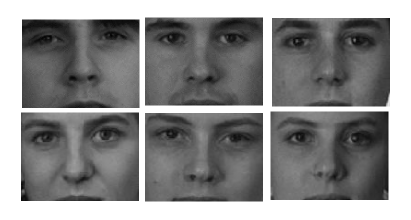
\includegraphics[width=\linewidth]{img/white.png}
		
		\column{.50\linewidth}
		\centering
			Black people faces
		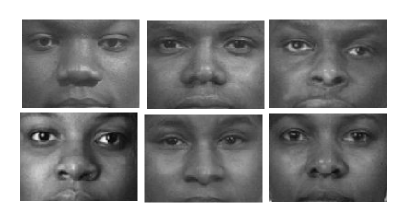
\includegraphics[width=\linewidth]{img/black.png}
	\end{columns}		
	\end{block}
	

	
	\begin{block}{16 Attribute stimuli}
		
	\begin{columns}[T]
	\begin{column}{.50\linewidth}
		\begin{center}
			\color{rasch}Positive attributes
		\end{center}
		
		Good, laughter, pleasure, glory, peace, happy, joy, love
	\end{column}
	
	\begin{column}{.50\linewidth}
		\begin{center}
			\color{alert}Negative attributes
		\end{center}
		
		Evil, bad, horrible, terrible, nasty, pain, failure, hate
	\end{column}
\end{columns}
	\end{block}
	\vspace{1.2mm}
	Participants: 62 (F $=48.39$\%, Age = $24.92\pm2.11$ years)

\end{frame}

\begin{frame}

\begin{block}{Two experimental conditions}
	\begin{columns}[T]
		\begin{column}{.50\linewidth}
			\begin{center}
				\textbf{White-Good/Black-Bad} (WGBB): 60 trials
			\end{center}
			
			\centering 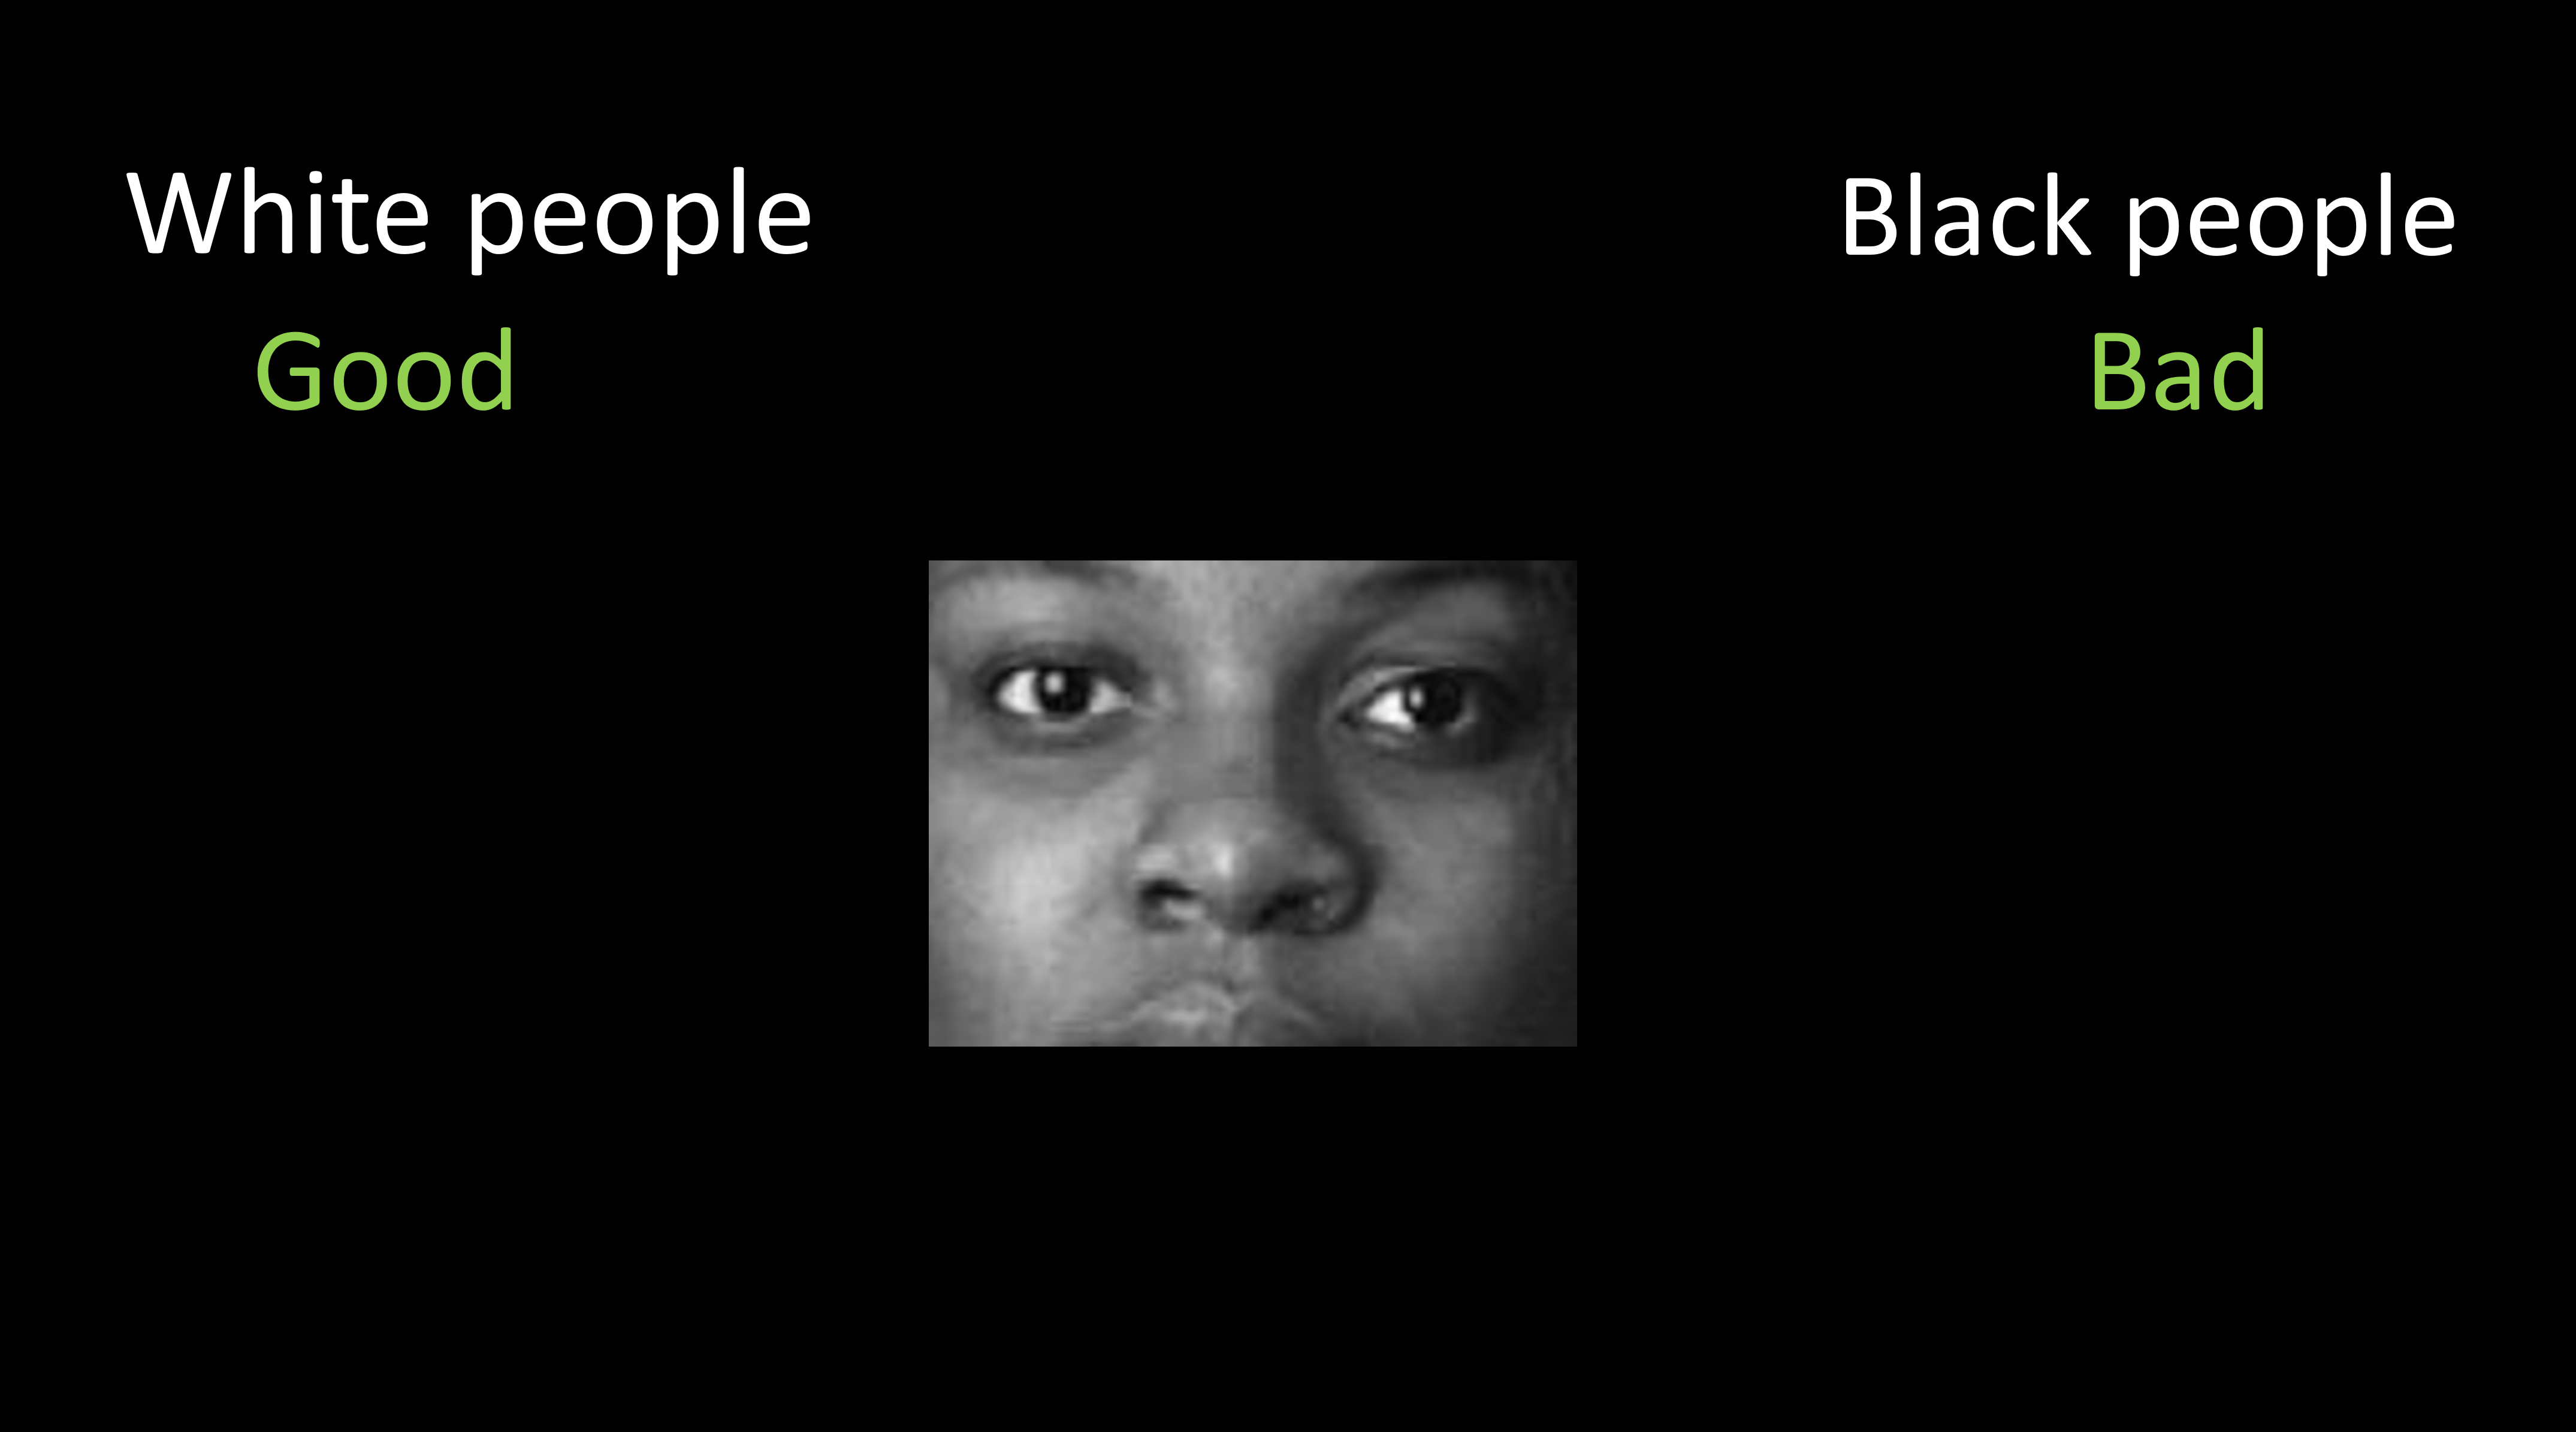
\includegraphics[width=\linewidth]{img/wgbb.png}
		\end{column}
		
		\begin{column}{.50\linewidth}
			\begin{center}
				\textbf{Black-Good/White-Bad} (BGWB):   60 trials
			\end{center}
			
			\centering 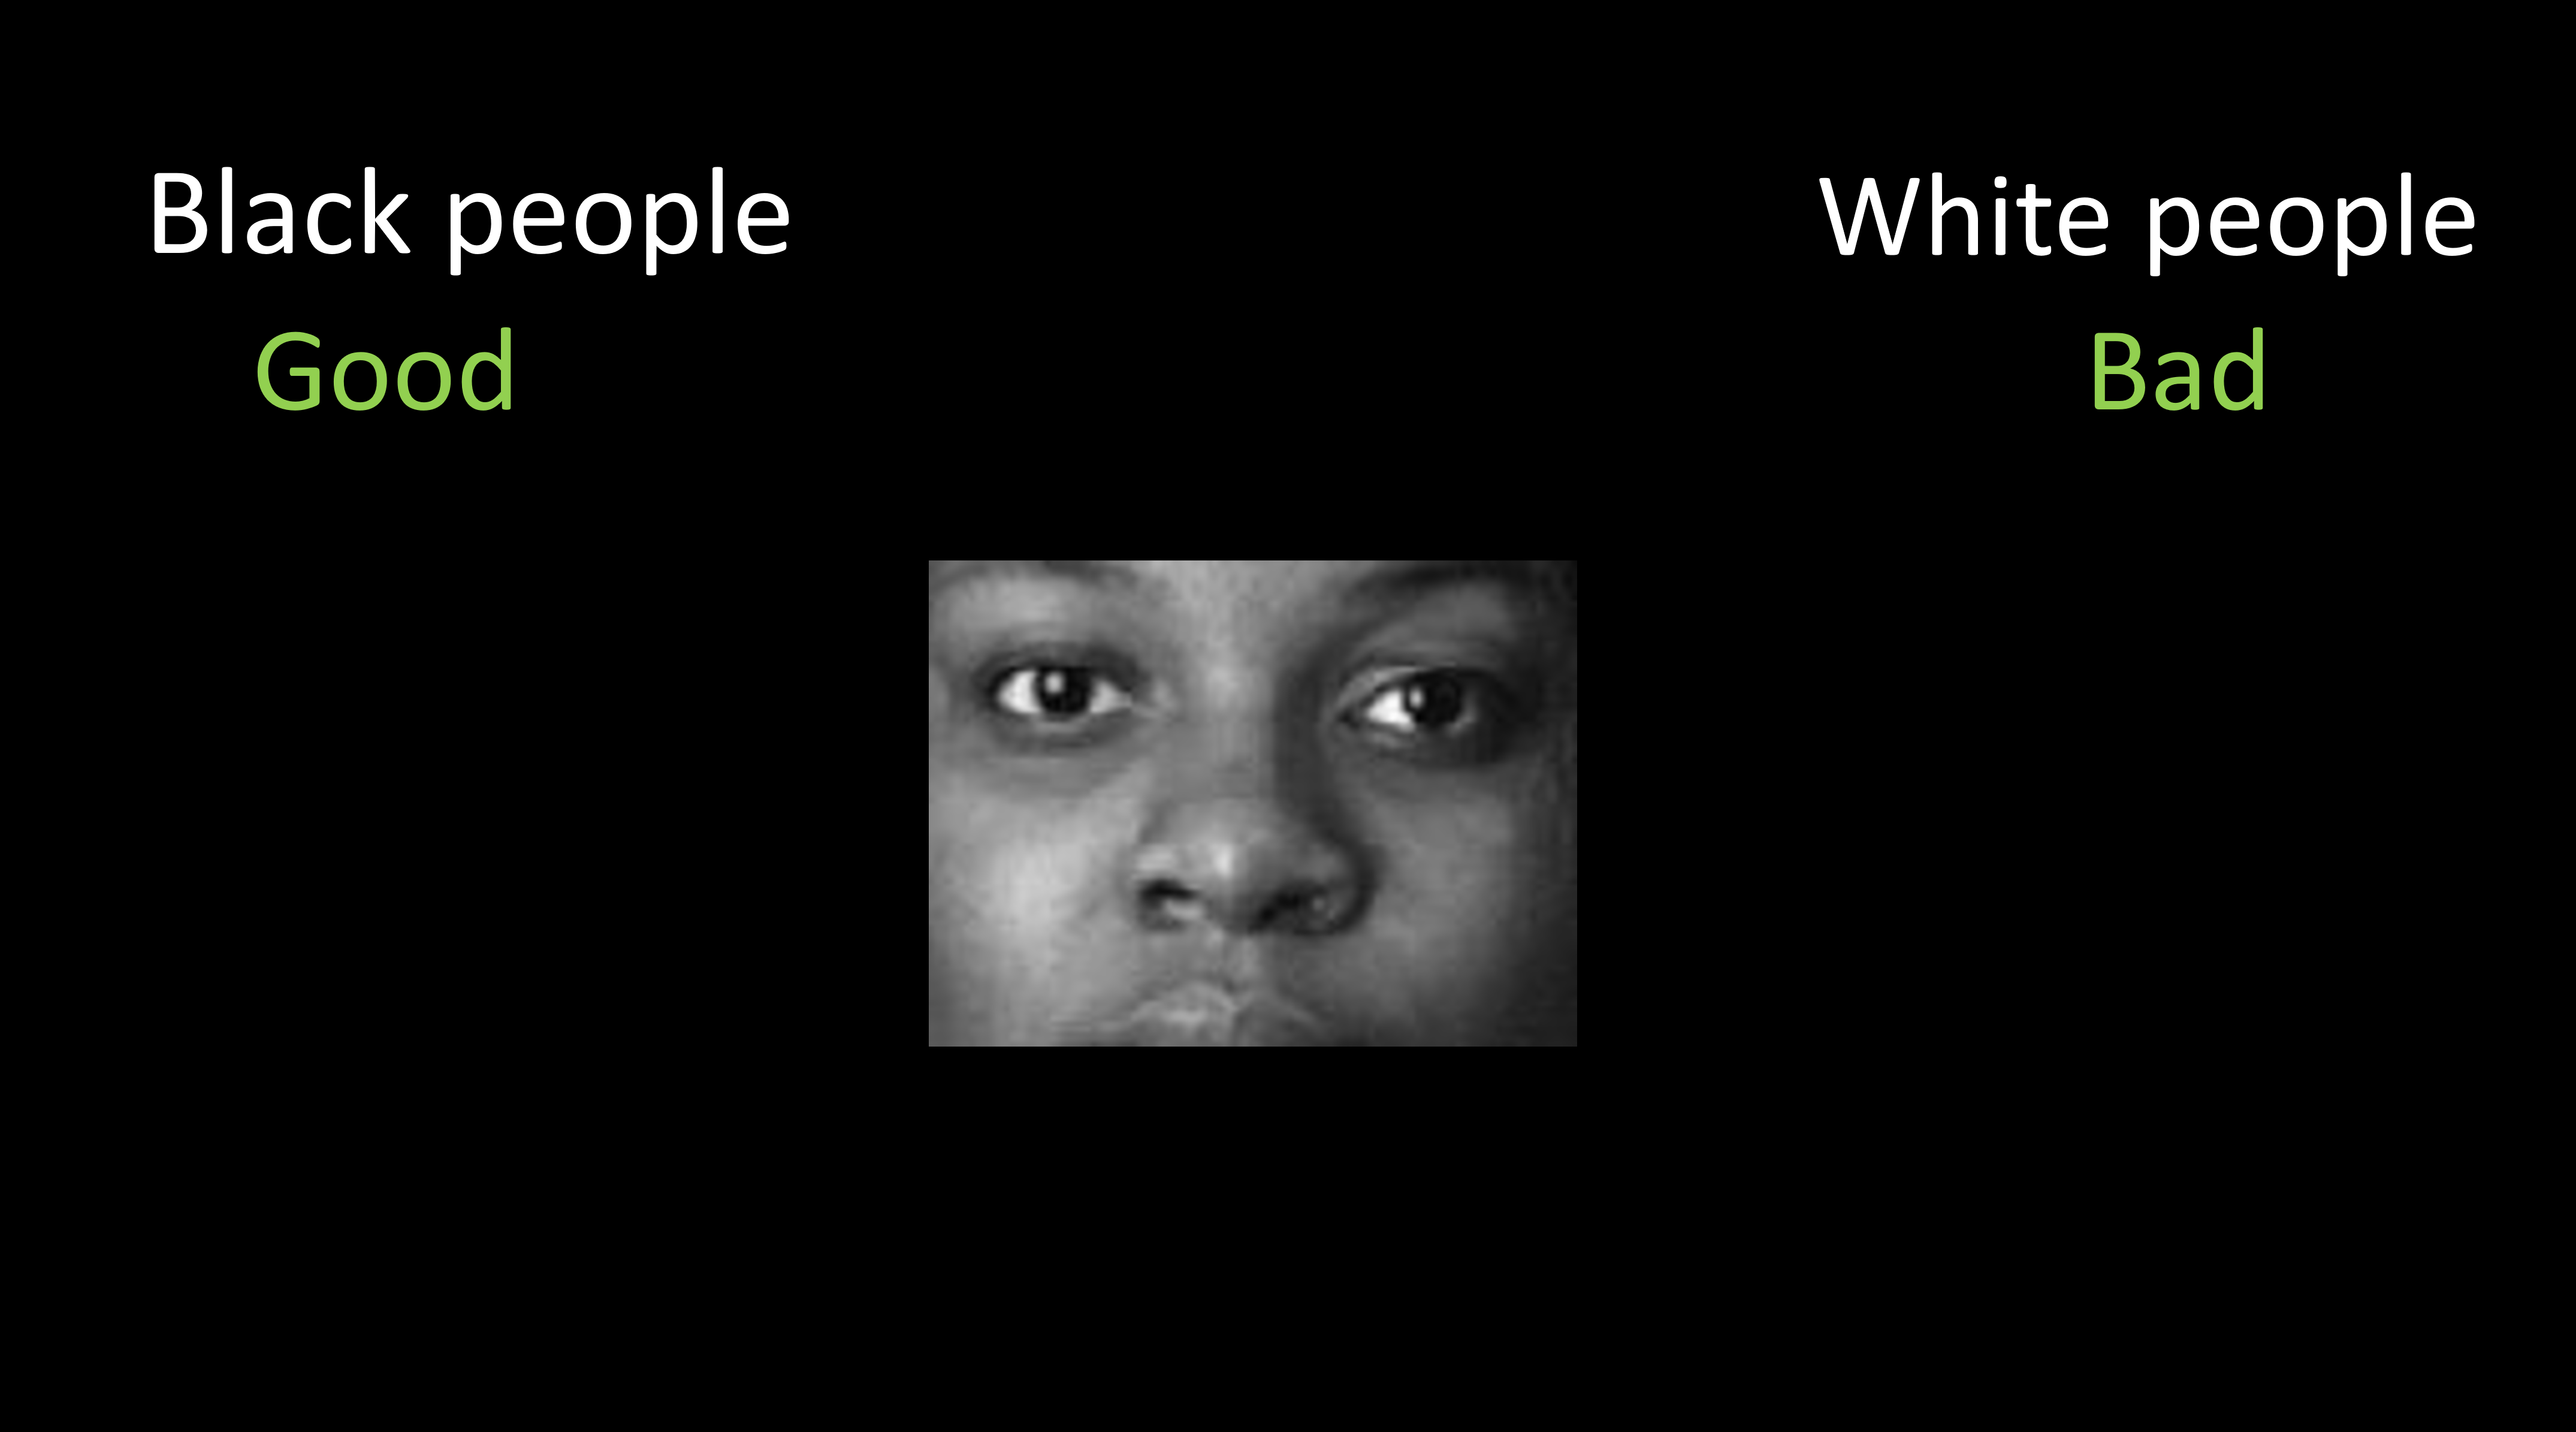
\includegraphics[width=\linewidth]{img/bgwb.png}
		\end{column}
	\end{columns}
\end{block}

\begin{equation*}
	D = \dfrac{M_{\text{BGWB}}-M_{\text{WGBB}}}{s_{\text{BGWB, WGBB}}}
\end{equation*}

\end{frame}

\subsection{Models}

\begin{frame}
	\begin{footnotesize}
		The expected response $y$ for the observation $i = 1, \ldots, I$ for respondent $p = 1,\ldots, P$ on stimulus $s = 1,\ldots, S$ in condition $c= 1,\ldots, C$:
	\end{footnotesize}
	\footnotesize
	
	
	\vspace{3mm}
	Model 1:
	\begin{equation*}\label{AccuracyMin}
		y_{i} = \spot<2->[fill =blue!15]{logit^{-1}(\alpha + \beta_c X_c}  + \spot<2->[fill=yellow!20]{\alpha_{p[i]} +  \alpha_{s[i]} + \varepsilon_{i})}
	\end{equation*}
	\begin{centering}
		
		$\alpha_p \sim \mathcal{N}(0, \sigma_p^2)$,
		
	\end{centering}
	
	\begin{centering}
		
		$\alpha_s \sim \mathcal{N}(0, \sigma_s^2)$.
		
	\end{centering}
	
	
	
	Model 2: 
	\begin{equation*}\label{Accuracy5}
		y_{i} = \spot<2->[fill =blue!15]{logit^{-1}(\alpha + \beta_c X_c}  + \spot<2->[fill=yellow!20]{ \alpha_{p[i]} +  \beta_{s[i]}c_{i} + \varepsilon_{i})}
	\end{equation*}
	
	\begin{centering}
		$\alpha_p \sim \mathcal{N}(0, \sigma_p^2)$,
		
	\end{centering}
	
	\begin{centering}
		
		$\beta_s \sim \mathcal{MVN}(0, \Sigma_{sc})$.
		
	\end{centering}
	
	Model 3: 
	
	\begin{equation*}
		y_{i} = \spot<2->[fill =blue!15]{logit^{-1}(\alpha + \beta_c X_c}  + \spot<2->[fill=yellow!20]{\alpha_{s[i]} +  \beta_{p[i]}c_{i} + \varepsilon_{i})}
	\end{equation*}
	
	\begin{centering}
		$\alpha_s \sim \mathcal{N}(0, \sigma_s^2)$,
		
	\end{centering}
	
	\begin{centering}
		
		$\beta_p \sim \mathcal{MVN}(0, \Sigma_{pc})$.
		
	\end{centering}
	
	
	\vspace{1.5mm}
	
	\footnotesize{Accuracy: $\epsilon \sim Logistic (0, \sigma^2)$}
	
		\vspace{1.5mm}
\pause
\begin{columns}[T]
	\begin{column}{.50\linewidth}
		\centering
		
		\spot[fill = blue!15]{Fixed Effects}
		
	\end{column}
		\begin{column}{.50\linewidth}
				\centering
	
		\spot[fill = yellow!20]{Random structure}
	\end{column}
\end{columns}
\end{frame}

\subsection{Results}

\begin{frame}{Model 2 is the least wrong model}
	%	{\centering{\color{rasch}{Rasch model:}} \\ \small{Model 2} \\}
	
		\begin{equation*}\label{Accuracy5}
		y_{i} = logit^{-1}(\alpha + \beta_c X_c +  \alpha_{p[i]} +  \beta_{s[i]}c_{i} + \varepsilon_{i})
	\end{equation*}
	
	\centering
	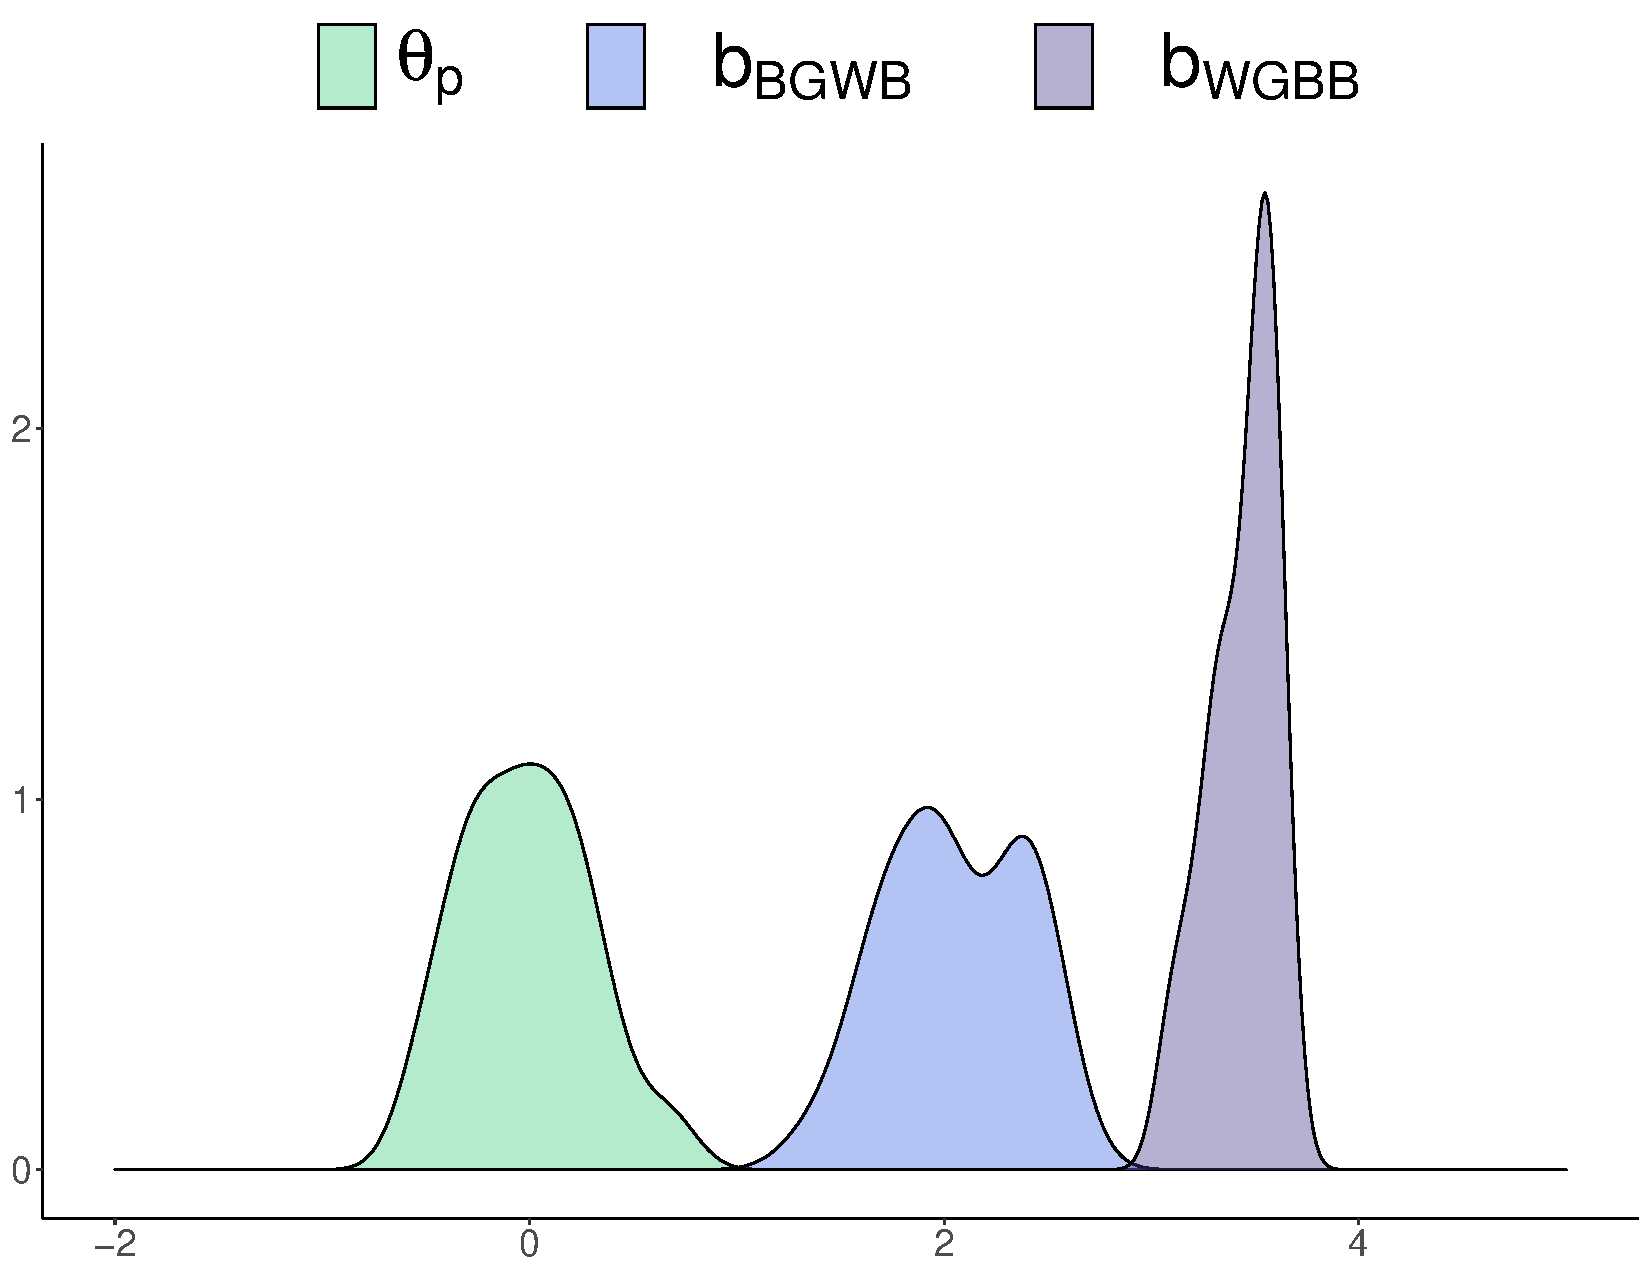
\includegraphics[width=0.6\linewidth]{img/raceParaccuracy.pdf}
\end{frame}

\begin{frame}{Condition--specific easiness}
	
	\vspace{7mm}
	\begin{columns}
		
		\column{.55\linewidth}
		\centering{\textcolor{comp}{\textsc{Highly contributing stimuli}}}
		
		\vspace{5mm}
		\onslide<1->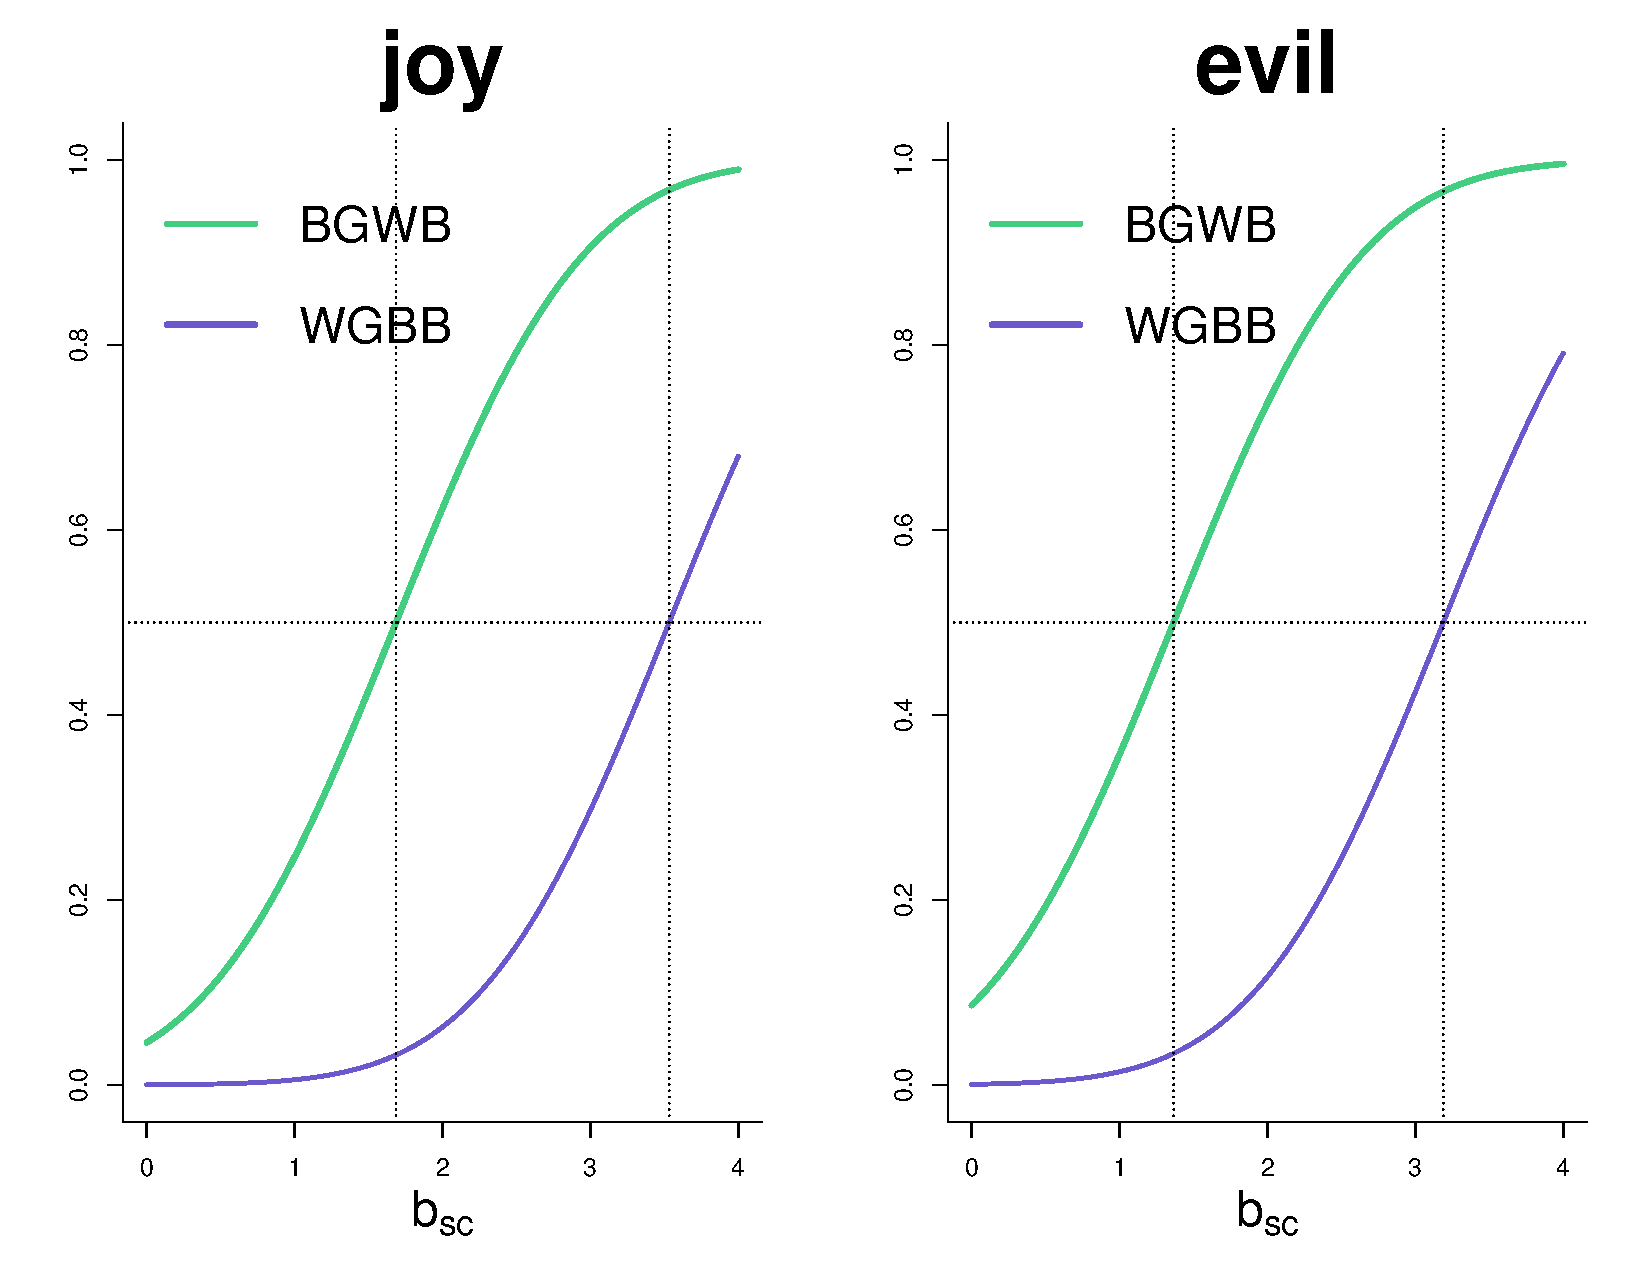
\includegraphics[width=\textwidth]{img/RaceHigh.pdf}
		
		\column{.55\linewidth}
		\centering{\textcolor{inc}{\textsc{Lowly contributing stimuli}}}
		
		\vspace{5mm}
		\onslide<1->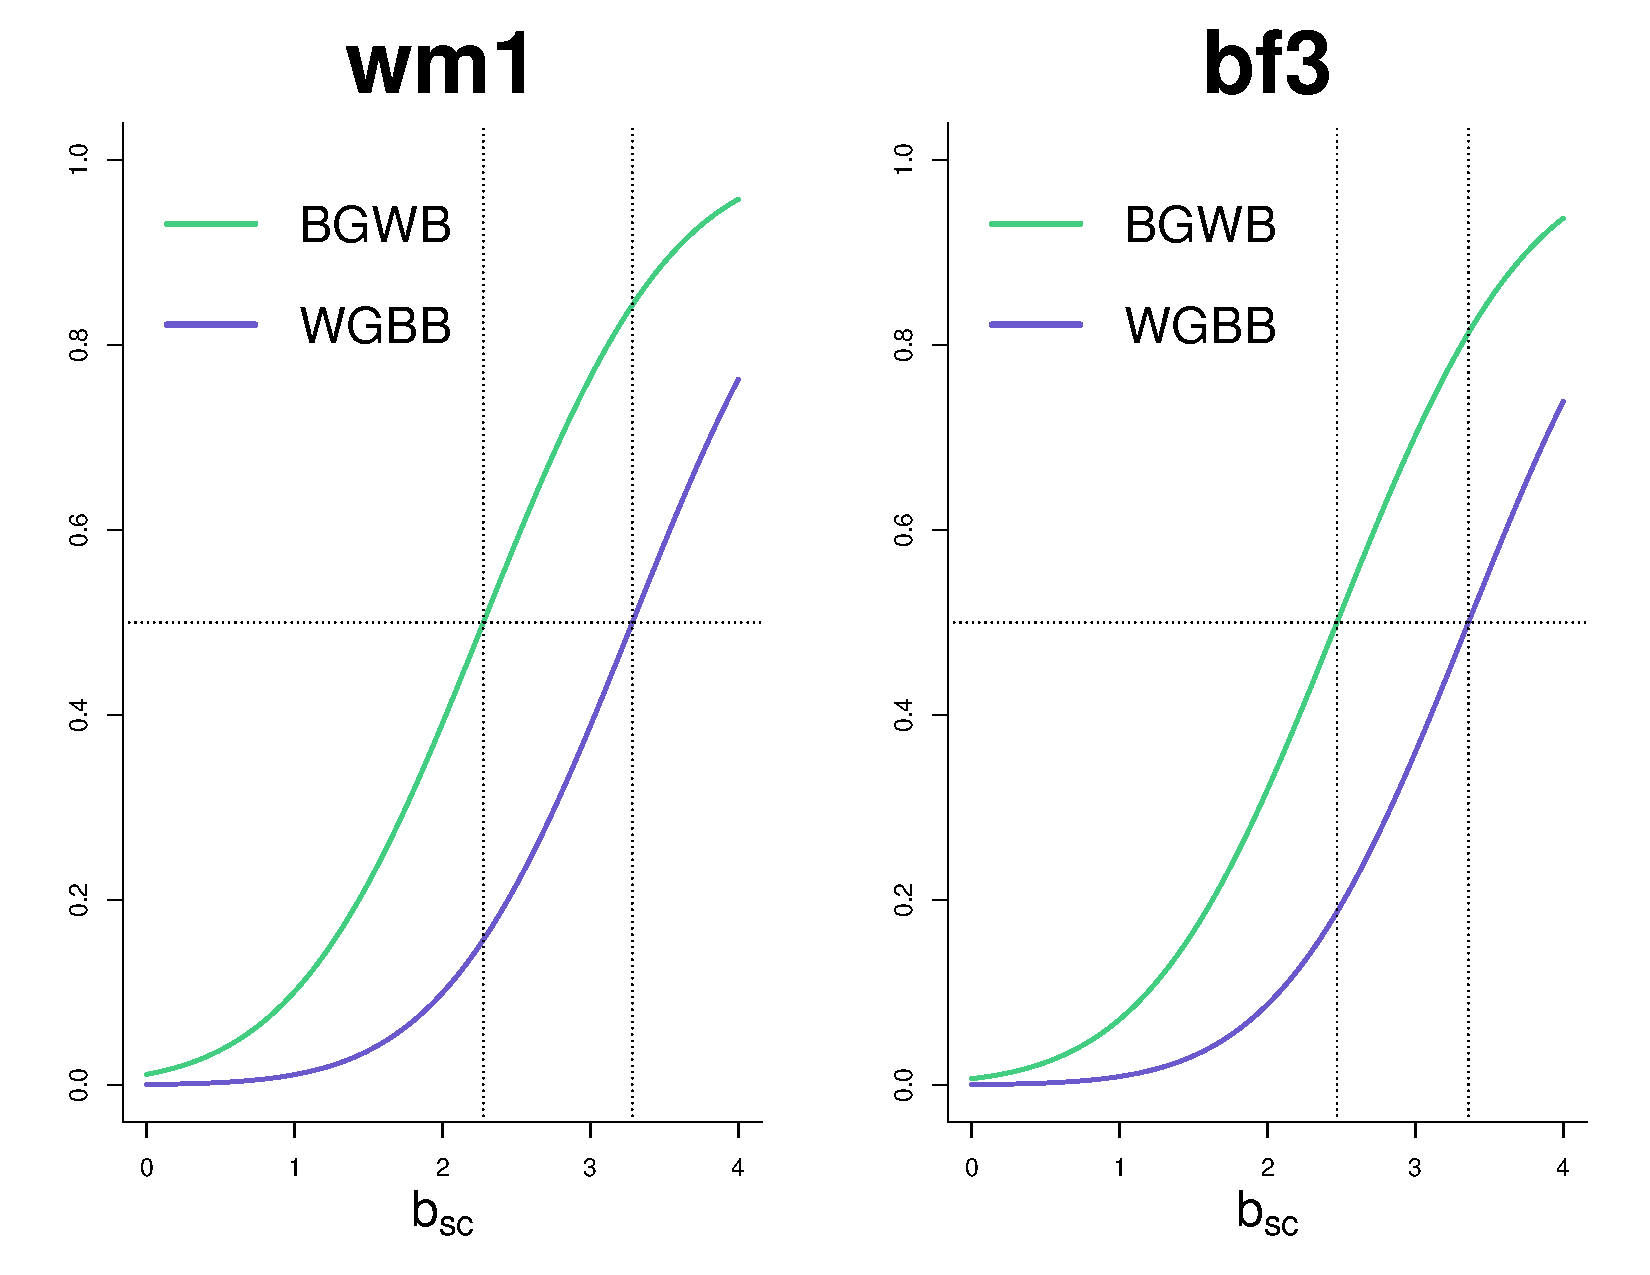
\includegraphics[width=\textwidth]{img/RaceLow.pdf}
	\end{columns}
	\tikzoverlay (n1) at (7.cm, 5.3cm){%
		\begin{minipage}{0.12\linewidth}
			\centering	
\includegraphics[width=0.65\linewidth]{img/wm1.jpg}
		\end{minipage}
	}; %
	\tikzoverlay (n2) at (10cm, 5.3cm){%
		\begin{minipage}{0.12\linewidth}
			\centering	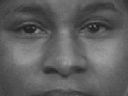
\includegraphics[width=0.65\linewidth]{img/bf56.jpg}
		\end{minipage}
	}; %
	%\vspace{\fill}
\end{frame}

\section{Discussion}

\begin{frame}
	\begin{itemize}
		\item Acknowledge and gather the information at the stimulus level
	\item Improve generalizability of the results to other sets of stimuli 

\item Control for random variance in the data 

\item Allow for obtaining a Rasch-like parametrization of the data 

\item Possibility of extending the (linear) model to other dependent variables (e.g., response times)
		
	\end{itemize}
\end{frame}


\begin{frame}
	\begin{center}
		\begin{Large}
			Thank you!
		\end{Large}
		
		ottavia.epifania@unipd.it
	\end{center}
	
	
\end{frame}
\end{document}
